\documentclass{article}
\usepackage{graphicx} % Required for inserting images

\usepackage[utf8]{inputenc}
\usepackage{algorithm}
\usepackage{algpseudocode}

\usepackage{amsmath, amsthm, amssymb}
\usepackage{amsfonts}
\usepackage{mathrsfs}

% Define the warning command
\newcommand{\warning}{{\fontencoding{U}\fontfamily{futs}\selectfont\char 49\relax} \ }




\usepackage{environ}

\usepackage{amsthm}
\usepackage{etoolbox} % Required for \AtBeginEnvironment and \AtEndEnvironment

\theoremstyle{definition}

\newtheorem{definition}{Definition}[section]
\AtBeginEnvironment{definition}{%
  \pushQED{\qed}\renewcommand{\qedsymbol}{$\diamondsuit$}%
}
\AtEndEnvironment{definition}{\popQED}

\newtheorem{theorem}{Theorem}[section]
\AtBeginEnvironment{theorem}{%
  \pushQED{\qed}\renewcommand{\qedsymbol}{$\spadesuit$}%
}
\AtEndEnvironment{theorem}{\popQED}

\newtheorem{lemma}{Lemma}[section]
\AtBeginEnvironment{lemma}{%
  \pushQED{\qed}\renewcommand{\qedsymbol}{\rotatebox[origin=c]{180}{$\spadesuit$}}%
}
\AtEndEnvironment{lemma}{\popQED}

\newtheorem{conjecture}{Conjecture}[section]
\AtBeginEnvironment{conjecture}{%
  \pushQED{\qed}\renewcommand{\qedsymbol}{$\clubsuit$}%
}
\AtEndEnvironment{conjecture}{\popQED}

% Define the 'remark' environment with specific ending
\newtheorem*{remark}{Remark}
\AtBeginEnvironment{remark}{%
  \pushQED{\qed}\renewcommand{\qedsymbol}{$\triangle$}%
}
\AtEndEnvironment{remark}{\popQED}

\newtheorem{proofsketch}{ProofScetch}[section]
\AtBeginEnvironment{proofsketch}{%
  \pushQED{\qed}\renewcommand{\qedsymbol}{\rotatebox[origin=c]{180}{$\heartsuit$}}%
}
\AtEndEnvironment{lemma}{\popQED}

\renewcommand\qedsymbol{\textbf{Q.E.D.} \  $\heartsuit$}








\usepackage{hyperref}

\usepackage[backref=true]{biblatex}
\addbibresource{ref.bib}

% https://tex.stackexchange.com/questions/159669/how-to-print-a-warning-sign-triangle-with-exclamation-point
%\usepackage{fourier}

\usepackage[toc,page]{appendix}

\title{Dominating mixed actions \\ in random matrices \\ (Draft version)}
\author{József Konczer}
\date{August 2024}

\begin{document}

\maketitle

\begin{abstract}
    This work has two main objectives: i.) it aims to derive the probability of the event when there exists a mixing ratio $p$, by which the mixture of the first two rows can dominate all other rows in a $N \times M$ Gaussian random utility matrix; ii.) it introduces a general, powerful, but still experimental technique, termed the ``continuous inclusion-exclusion principle,'' by which an integral formula can be obtained. The results based on the ``continuous inclusion-exclusion principle'' are matched with more elementary calculations in special cases, and the results are also compared with numerical Monte Carlo simulations.
\end{abstract}

\section{Introduction}

We will assume that we have random utility matrices from a
real gaussian matrix ensemble \cite{book:RandomMatrix}

\begin{equation}
    U_{i,j} \sim \mathcal{N}(0,1), \quad i \in \{1,\dots,N\}, j \in \{1,\dots,M\}
\end{equation}

We call the first and second actions a dominating pair (being able to form a ``strictly dominant mixed strategy'' \cite{book:GameTheory101} in the context of Game Theory \cite{book:EssentialGameTheory,book:GameTheory}), iff:

\begin{equation}
    \exists p \in [0,1],  \forall j \in \{1,\dots,M\}, k \in \{3,\dots,N\} \quad p \ U_{1,j} + (1-p) \ U_{2,j} > U_{k,j} 
\end{equation}

We introduce several events: $E_j(p)$ is the event that in the $j$-th column, the mixture of the first and second element with mixing ratio $p$ dominates all other entries in that column:

\begin{equation}
    E_j(p) = \{ p \ u_{1,j} + (1-p) \ u_{2,j} > \max(u_{3,j},\dots,u_{N,j}) \ | \ u_{i,j} \in \mathbb{R}\}
\end{equation}

$E(p)$ is the event that in all columns, the mixture of the first and second rows with the same mixing ratio $p$ will dominate all further rows:

\begin{equation}
    E(p) = \bigcap_{j=1}^M E_j(p)
\end{equation}

Finally, $E$ is the event that there is a $p\in[0,1]$ mixing ratio, by which the mixture of the first and second row can dominate all other rows:

\begin{equation}
    E = \bigcup_{p \in [0,1]} E(p)
\end{equation}

In the following sections, our main goal is to calculate the chance of $E$ happening, i.e. $\Pr(E)$ as a function of $N$ and $M$.

\section{Continuous inclusion-exclusion principle}


\warning
Now we spell out a conjecture, which does not follow from the $\sigma$- (or complete) additivity of probability measures \cite{book:Kolmogorov,book:Renyi1970} (which guarantees the measurability of countable collections of measurable sets). We call the formula
``Continuous inclusion-exclusion principle'':

\begin{equation}
\label{eq:CIEP}
    \Pr(E) = \lim_{L \to \infty} \sum_{n=1}^\infty (-1)^{n-1} L^n
    \underset{0 \le p_1 < \dots < p_n \le 1}{\int\dots\int}
    \Pr \left ( 
    \bigcap_{k=1}^n E(p_k)
    \right ) 
    dp_1\dots dp_n
\end{equation}

As the name suggests, this can be viewed as the generalization of the finite (or at least countable) inclusion-exclusion principle to a continuum union of measurable sets.

Assuming $0\le p_1<\dots<p_n\le 1$, the probability of the intersection of events $E(p_i)$ simplify, because if two (or more) (possibly mixed-)actions are dominating, then any convex combination is also dominating. 

\begin{equation}
    \Pr \left ( 
    \bigcap_{k=1}^n E(p_k)
    \right ) 
    =
    \Pr \left (
    E(p_1) \cap E(p_n)
    \right )
    =
    F(p_1,p_n)
\end{equation}

Formally, we can express the probability of single events using $F(.,.)$:

\begin{equation}
    \Pr(E(p)) = F(p,p)
\end{equation}

Therefore, for all $n\ge 2$ we have:

\begin{equation}
    \underset{0 \le p_1 < \dots < p_n \le 1}{\int\dots\int}
    \Pr \left ( 
    \bigcap_{k=1}^n E(p_k)
    \right ) 
    dp_1\dots dp_n
    =
    \iint\limits_{0 \le p_1 < p_n \le 1}
    \frac{(p_n-p_1)^{n-2}}{(n-2)!}
    F(p_1,p_n) \ dp_1 dp_n
\end{equation}

Therefore:

\begin{equation}
 \Pr(E) = \lim_{L \to \infty} 
    \left (
    L \int_{0}^1 \Pr(E(p)) \ dp + 
    \sum_{n=2}^\infty (-1)^{n-1} L^n
    \iint\limits_{0 \le p_1 < p_n \le 1}
    \frac{(p_n-p_1)^{n-2}}{(n-2)!}
    F(p_1,p_n) \ dp_1 dp_n
    \right )
\end{equation}

\warning Interchanging summation and integration gives:

\begin{equation}
 \Pr(E) = \lim_{L \to \infty} 
    \left (
    L \int_{0}^1 F(p,p) \ dp + 
    \iint\limits_{0 \le p'_1 < p'_2 \le 1}
    \sum_{n=2}^\infty (-1)^{n-1} L^n
    \frac{(p'_2-p'_1)^{n-2}}{(n-2)!}
    F(p'_1,p'_2) \ dp'_1 dp'_2
    \right )
\end{equation}

The infinite sum yields an exponential function:

\begin{equation}
 \Pr(E) = \lim_{L \to \infty} 
    \left (
    L \int_{0}^1 F(p,p) \ dp - 
    L^2
    \iint\limits_{0 \le p'_1 < p'_2 \le 1}
    e^{-L (p'_2-p'_1)}
    F(p'_1,p'_2) \ dp'_1 dp'_2
    \right )
\end{equation}

To progress with the calculation, we implement the following change of variables to ``center of mass coordinates'':

\begin{equation}
    \overline{p}= \frac{p'_1+p'_2}{2}, \quad
    \Delta = p'_2-p'_1
\end{equation}

\begin{equation}
    p'_1 = \overline{p} - \Delta/2, \quad
    p'_2 = \overline{p} + \Delta/2
\end{equation}

And we introduce the following integration limits for $\Delta$:

\begin{equation}
    \hat{\Delta}(\overline{p}) = 2 \ \min(\overline{p},1-\overline{p})
\end{equation}

The Jacobian looks the following:

\begin{equation}
    J = \frac{\partial (p'_1,p'_2)}{\partial (\overline{p},\Delta)} =
    \begin{pmatrix}
    1 & 1 \\
    -1/2 & 1/2
    \end{pmatrix}
\end{equation}

It has a unit determinant:

\begin{equation}
    |J| = 1
\end{equation}

The two-dimensional integral looks the following in these new variables:

\begin{equation}
    G(L)
    =
    \iint\limits_{0 \le p'_1 < p'_2 \le 1}
    e^{-L (p'_2-p'_1)}
    F(p'_1,p'_2) \ dp'_1 dp'_2
\end{equation}

\begin{equation}
    G(L)
    =
    \int_0^1 \int_0^{\hat{\Delta}(\overline{p})} e^{- L \Delta} 
    F(\overline{p} - \Delta/2, \overline{p} + \Delta/2) 
    \ d\Delta d\overline{p}
\end{equation}

First, let us evaluate the following integral:

\begin{equation}
    I(\overline{p},L)
    =
    \int_0^{\hat{\Delta}(\overline{p})} e^{- L \Delta} 
    F(\overline{p} - \Delta/2, \overline{p} + \Delta/2) 
    \ d\Delta 
\end{equation}

Integration by parts results:

\begin{equation}
    I(\overline{p},L)
    =
    \left [
    \frac{e^{- L \Delta}}{- L} 
    F(\overline{p} - \Delta/2, \overline{p} + \Delta/2) 
    \right ]_{\Delta=0_+}^{\hat{\Delta}(\overline{p})}
    -
    \int_0^{\hat{\Delta}(\overline{p})}
    \frac{e^{- L \Delta}}{- L} 
    \frac{\partial
    F(\overline{p} - \Delta/2, \overline{p} + \Delta/2) 
    }{\partial \Delta}
    \ d \Delta
\end{equation}

Introducing a ``second order'' integral gives:

\begin{equation}
    I_2(\overline{p},L)
    =
    (-1)
    \int_0^{\hat{\Delta}(\overline{p})}
    \frac{e^{- L \Delta}}{- L} 
    \frac{\partial
    F(\overline{p} - \Delta/2, \overline{p} + \Delta/2) 
    }{\partial \Delta}
    \ d \Delta
\end{equation}

Where we can use integration by parts one more time:

\begin{equation}
    I_2(\overline{p},L)
    =
    (-1)
    \left [
    \frac{e^{- L \Delta}}{(- L)^2} 
    \frac{\partial
    F(\overline{p} - \Delta/2, \overline{p} + \Delta/2) 
    }{\partial \Delta}
    \right ]_{\Delta=0_+}^{\hat{\Delta}(\overline{p})}
    -
    (-1)
    \int_0^{\hat{\Delta}(\overline{p})}
    \frac{e^{- L \Delta}}{(- L)^2} 
    \frac{\partial^2
    F(\overline{p} - \Delta/2, \overline{p} + \Delta/2) 
    }{\partial^2 \Delta}
    \ d \Delta
\end{equation}

Introducing a ``third order'' integral gives:

\begin{equation}
    I_3(\overline{p},L)
    =
    (-1)^2
    \int_0^{\hat{\Delta}(\overline{p})}
    \frac{e^{- L \Delta}}{(- L)^2} 
    \frac{\partial^2
    F(\overline{p} - \Delta/2, \overline{p} + \Delta/2) 
    }{\partial^2 \Delta}
    \ d \Delta
\end{equation}

Using the previous results, the two-dimensional integral $G(L)$ can be expanded to three terms -- from which two will give a contribution -- and a reminder term:

\begin{equation}
    G(L) = G_1(L) + G_2(L) + \mathcal{R}_3(L)
\end{equation}

\begin{equation}
    G_1(L)
    =
    \int_0^1  
    \left [
    \frac{e^{- L \Delta}}{- L} 
    F(\overline{p} - \Delta/2, \overline{p} + \Delta/2) 
    \right ]_{\Delta=0}^{\hat{\Delta}(\overline{p})}
    \ d\overline{p}
\end{equation}

\begin{equation}
    G_2(L)
    =
    \int_0^1  
    (-1)
    \left [
    \frac{e^{- L \Delta}}{(- L)^2} 
    \frac{\partial
    F(\overline{p} - \Delta/2, \overline{p} + \Delta/2) 
    }{\partial \Delta}
    \right ]_{\Delta=0}^{\hat{\Delta}(\overline{p})}
    \ d\overline{p}
\end{equation}

\begin{equation}
    \mathcal{R}_3(L)
    =
    \int_0^1 
    I_3(\overline{p},L)
    \  d \overline{p}
    =
    \int_0^1 \int_0^{\hat{\Delta}(\overline{p})}
    \frac{e^{- L \Delta}}{(- L)^2} 
    \frac{\partial^2
    F(\overline{p} - \Delta/2, \overline{p} + \Delta/2) 
    }{\partial^2 \Delta}
    \ d \Delta d \overline{p}
\end{equation}

\begin{lemma}

If the second derivative of $F$ with respect to $\Delta$ is bounded on the integration domain $\mathcal{D}$:

\begin{equation}
    \mathcal{D} = \{ (\overline{p},\Delta) \ | \ \Delta \in [0, \hat{\Delta}(\overline{p})], \overline{p} \in [0, 1] \}
\end{equation}

i.e.

\begin{equation}
    \frac{\partial^2
    F(\overline{p} - \Delta/2, \overline{p} + \Delta/2) 
    }{\partial^2 \Delta}
    \in
    B(\mathcal{D})
\end{equation}

Then the reminder term is in $\mathcal{O}(L^{-3})$ class:

\begin{equation}
    \mathcal{R}_3(L) = \mathcal{O}(L^{-3})
\end{equation}

\end{lemma}



\begin{proof}

$\frac{\partial^2 F(\overline{p} - \Delta/2, \overline{p} + \Delta/2) }{\partial^2 \Delta}$ is Bounded, therefore:

\begin{equation}
    \exists M_2 \in \mathbb{R}, \forall (\overline{p},\Delta) \in \mathcal{D}, \quad
    \left |
    \frac{\partial^2
    F(\overline{p} - \Delta/2, \overline{p} + \Delta/2) 
    }{\partial^2 \Delta}
    \right | \le M_2
\end{equation}

Straightforward calculation gives that:

\begin{equation}
    \iint\limits_\mathcal{D} e^{-L \Delta} \ d \Delta d \overline{p}
    =
    \frac{1}{L} - \frac{2}{L^2} + 2 \frac{e^{-L/2}}{L}
    =
    \mathcal{O}(L^{-1})
\end{equation}

Therefore, simply by applying Hölder's inequality \cite{book:Holder} we get:

\begin{equation}
    \left |
    \iint\limits_\mathcal{D} 
    \frac{e^{- L \Delta}}{(- L)^2} 
    \frac{\partial^2
    F(\overline{p} - \Delta/2, \overline{p} + \Delta/2) 
    }{\partial^2 \Delta}
    \ d \Delta d \overline{p}
    \right |
    \le
    M_2 
    \left ( 
    \frac{1}{L^3} - \frac{2}{L^4} + 2 \frac{e^{-L/2}}{L^3}
    \right )
    =
    \mathcal{O}(L^{-3})
\end{equation}

Therefore:

\begin{equation}
    |\mathcal{R}_3(L)| \le \mathcal{O}(L^{-3})
\end{equation}

\end{proof}

Now we can determine the contributions from $G_1(L)$. The first order part can be split into contributions from the upper and lower limits:

\begin{equation}
    G_1(L) = G_A(L) + G_B(L)
\end{equation}

The contribution from the lower limit ($\Delta=0$) is easy to determine:

\begin{equation}
    G_A(L) 
    =
    -
    \int_0^1  
    \frac{e^{- L \cdot 0}}{- L} 
    F(\overline{p} - 0/2, \overline{p} + 0/2) 
    \ d\overline{p}
    =
    \frac{1}{L} 
    \int_0^1  
    F(\overline{p}, \overline{p}) 
    \ d\overline{p}
\end{equation}

While integrating the contribution from the upper limit needs more consideration (here we split the integration domain into two to simplify the formula for $\hat{\Delta}(\overline{p})$):

\begin{equation}
    G_B(L)
    =
    \int_0^{1/2} 
    \frac{e^{- L 2 \overline{p}}}{- L} 
    F(0, 2 \ \overline{p})
    \ d \overline{p} +
    \int_{1/2}^{1} 
    \frac{e^{- L 2 (1-\overline{p})}}{- L} 
    F(2 \ \overline{p} - 1, 1)
    \ d \overline{p}
\end{equation}

Integration by parts gives:

\begin{equation}
    \int_0^{1/2} 
    \frac{e^{- L 2 \overline{p}}}{- L} 
    F(0, 2 \ \overline{p})
    \ d \overline{p}
    =
    \left [
    \frac{e^{- L 2 \overline{p}}}{2 \ (- L)^2} 
    F(0, 2 \ \overline{p})
    \right ]_{\overline{p}=0}^{1/2}
    -
    \int_0^{1/2} 
    \frac{e^{- L 2 \overline{p}}}{2 \ (- L)^2} 
    \frac{\partial F(0, 2 \ \overline{p})}{\partial \overline{p}}
    \ d \overline{p}
\end{equation}

We can split the integral into a part which will have a remaining contribution and a reminder term:

\begin{equation}
    \int_0^{1/2} 
    \frac{e^{- L 2 \overline{p}}}{- L} 
    F(0, 2 \ \overline{p})
    \ d \overline{p}
    =
    -\frac{1}{2} \frac{1}{L^2} 
    F(0, 0) +
    \mathcal{R}_{B,1}
\end{equation}

The remainder being:

\begin{equation}
    \mathcal{R}_{B,1}
    =
    \frac{e^{- L }}{2 \ L^2} 
    F(0, 1) -
    \int_0^{1/2} 
    \frac{e^{- L 2 \overline{p}}}{2 \ (- L)^2} 
    \frac{\partial F(0, 2 \ \overline{p})}{\partial \overline{p}}
    \ d \overline{p}
\end{equation}

We can see by recalling Hölder's inequality that if $\frac{\partial F(0, 2 \ \overline{p})}{\partial \overline{p}}$ is bounded on $\overline{p} \in [0,1/2]$ interval, then:

\begin{equation}
    |\mathcal{R}_{B,1}|
    \le
    \mathcal{O}(L^{-3})
\end{equation}

In a similar spirit we get (if $\frac{\partial F(2 \ \overline{p} - 1,1)}{\partial \overline{p}}$ is bounded on $\overline{p} \in [1/2,1]$ interval) that:

\begin{equation}
    \int_{1/2}^{1} 
    \frac{e^{- L 2 (1-\overline{p})}}{- L} 
    F(2 \ \overline{p} - 1, 1)
    \ d \overline{p}
    =
    -\frac{1}{2} \frac{1}{L^2} 
    F(1, 1) +
    \mathcal{R}_{B,2}
\end{equation}

\begin{equation}
    \mathcal{R}_{B,2}
    =
    \frac{e^{- L }}{2 \ L^2} 
    F(0, 1) -
    \int_{1/2}^{1} 
    \frac{e^{- L 2 (1-\overline{p})}}{2 \ (- L)^2} 
    \frac{\partial F(2 \ \overline{p} - 1, 1)}{\partial \overline{p}}
    \ d \overline{p}
\end{equation}

\begin{equation}
    |\mathcal{R}_{B,2}|
    \le
    \mathcal{O}(L^{-3})
\end{equation}

Collecting all terms together, we get:

\begin{equation}
    G_B(L) = 
    -\frac{1}{2} \frac{1}{L^2} 
    F(0, 0) 
    -\frac{1}{2} \frac{1}{L^2} 
    F(1, 1) +
    \mathcal{R}_B
\end{equation}

\begin{equation}
    \mathcal{R}_B
    =
    \mathcal{R}_{B,1} + \mathcal{R}_{B,2}
\end{equation}

Now we can proceed with $G_2(L)$. Splitting it into two contributions from lower and upper bounds we get:

\begin{equation}
    G_2(L) = G_C(L) + G_D(L)
\end{equation}

The contribution from the lower bound ($\Delta=0_+$) is easy to determine:

\begin{equation}
    G_C(L) = -\frac{1}{L^2}
    \int_0^1
    \frac{\partial
    F(\overline{p} - \Delta/2, \overline{p} + \Delta/2) 
    }{\partial \Delta}
    \Bigg |_{\Delta=0_+}
    \ d\overline{p}
\end{equation}

While the contribution from the upper bound can be squeezed to a reminder term:

\begin{equation}
    G_D = \int_0^1 
    -
    \frac{e^{- L \hat{\Delta}(\overline{p})}}{L^2} 
    \frac{\partial
    F(\overline{p} - \Delta/2, \overline{p} + \Delta/2) 
    }{\partial \Delta}
    \Bigg |_{\Delta=\hat{\Delta}(\overline{p})}
    \ d\overline{p}
\end{equation}

\begin{equation}
    G_D = \mathcal{R}_D
\end{equation}

Again, recalling Hölder's inequality, we get that
if $\frac{\partial
    F(\overline{p} - \Delta/2, \overline{p} + \Delta/2) 
    }{\partial \Delta}
    \Big |_{\Delta=\hat{\Delta}(\overline{p})}$ is bounded, then:



\begin{equation}
    |\mathcal{R}_D|
    \le
    \mathcal{O}(L^{-3})
\end{equation}

Collecting the terms, we get the following expression for $\Pr(E)$:

\begin{equation}
 \Pr(E) = \lim_{L \to \infty} 
    \left (
    L \int_{0}^1 F(p,p) \ dp - 
    L^2 (G_A(L) + G_B(L) + G_C(L) + G_D(L) + \mathcal{R}_3(L))
    \right )
\end{equation}


\begin{equation}
\begin{split}
 \Pr(E) = \lim_{L \to \infty} 
    & \Big (
    L \int_{0}^1 F(p,p) \ dp + 
    \frac{1}{2} F(0,0) + \frac{1}{2} F(1,1)
    - L \int_{0}^1 F(\overline{p},\overline{p}) \ d\overline{p}
     \\
    &- \int_0^1
    \frac{\partial
    F(\overline{p} - \Delta/2, \overline{p} + \Delta/2) 
    }{\partial \Delta}
    \Bigg |_{\Delta=0_+}
    \ d\overline{p} +
    L^2 \ \mathcal{R}(L))
    \Big )
\end{split}
\end{equation}

\begin{equation}
    \mathcal{R}(L)
    =
    \mathcal{R}_B(L) +
    \mathcal{R}_D(L) +
    \mathcal{R}_3(L)
\end{equation}

Under mild regularity conditions mentioned previously, we have:

\begin{equation}
    \mathcal{R}(L)
    =
    \mathcal{O}(L^{-3})
\end{equation}

Therefore, the limit simplifies to:

\begin{equation}
\label{eq:PrE_Formula}
\boxed{
    \Pr(E) 
    = 
    \frac{1}{2} \left ( F(0,0)+F(1,1) \right ) 
    - \int_0^1
    \frac{\partial
    F(\overline{p} - \Delta/2, \overline{p} + \Delta/2) 
    }{\partial \Delta}
    \Bigg |_{\Delta=0_+}
    \ d\overline{p}
    }
\end{equation}

Or alternatively:

\begin{equation}
    \Pr(E) 
    = 
    \frac{1}{2} \left ( F(0,0)+F(1,1) \right ) 
    +
    \frac{1}{2}
    \int_0^1
    \left(
    \frac{\partial}{\partial p_1}-
    \frac{\partial}{\partial p_2}
    \right)
    F(p_1, p_2) 
    \Bigg |_{p_1=p_2=p}
    \ d p
\end{equation}

\begin{remark}[Parametrization invariance]
The expression for $\Pr(E)$ is invariant under the reparametrization of events $E(p)$ to $E(\vartheta)$:

For any differenciable monotone invertible biection $\vartheta(p)$, $p(\vartheta)$:

\begin{equation}
    p \to \vartheta
\end{equation}

\begin{equation}
    0 \to \vartheta_a, \quad
    1 \to \vartheta_b
\end{equation}


\begin{equation}
    \int_0^1
    \left(
    \frac{\partial}{\partial p_1}-
    \frac{\partial}{\partial p_2}
    \right)
    F(p_1, p_2) 
    \Bigg |_{p_1=p_2=p}
    \ d p
    =
    \int_{\vartheta_a}^{\vartheta_b}
    \left(
    \frac{d \vartheta_1}{d p_1} \frac{\partial}{\partial \vartheta_1}-
    \frac{d \vartheta_2}{d p_2} \frac{\partial}{\partial \vartheta_2}
    \right)
    F(\vartheta_1, \vartheta_2) 
    \Bigg |_{\vartheta_1=\vartheta_2=\vartheta}
    \frac{d p}{d \vartheta}\ d \vartheta
\end{equation}

Which simplifies to:

\begin{equation}
    \int_{\vartheta_a}^{\vartheta_b}
    \left(
    \frac{\partial}{\partial \vartheta_1}-
    \frac{\partial}{\partial \vartheta_2}
    \right)
    F(\vartheta_1, \vartheta_2) 
    \Bigg |_{\vartheta_1=\vartheta_2=\vartheta}
    \ d \vartheta
\end{equation}

Resulting:

\begin{equation}
    \Pr(E) 
    = 
    \frac{1}{2} \left ( F(\vartheta_a,\vartheta_a)+F(\vartheta_b,\vartheta_b) \right ) 
    - \int_{\vartheta_a}^{\vartheta_b}
    \frac{\partial
    F(\vartheta - \Delta/2, \vartheta + \Delta/2) 
    }{\partial \Delta}
    \Bigg |_{\Delta=0}
    \ d \vartheta
\end{equation}

This is expected because the definition of the event $E$ as a continuum union is independent of the parametrization of $E(.)$ events.
However, in the proposed general formula, all terms representing finite intersections are parametrization-dependent. Symmetry is restored only in the $ L \to \infty$ limit.

\end{remark}

\subsection{Calculating $F(.,.)$}

\subsubsection{Notation}

We will use standard notation for cumulative distribution function(s) for Gaussian random variables:

\begin{equation}
    \Phi(z) = \int_{-\infty}^z \frac{1}{\sqrt{2 \pi}} e^{-\frac{x^2}{2}} \ d x =
    \int_{-\infty}^z \varphi(x) \ d x
\end{equation}

\begin{equation}
    \Phi(z|\mu, \sigma^2) = \int_{-\infty}^z \frac{1}{\sqrt{2 \pi} \sigma} e^{-\frac{x^2}{2 \sigma^2}} \ d x =
    \int_{-\infty}^z \varphi(x|\mu,\sigma^2) \ d x
\end{equation}

We introduce a standard notation for complement probabilities:

\begin{equation}
    q_i = 1-p_i
\end{equation}

Introducing a mixture of Gaussian random variables:

\begin{equation}
    X_1(p_1,p_2) = p_1 \ U_{1,1} + q_1 \ U_{2,1}, \quad
    X_2(p_1,p_2) = p_2 \ U_{1,1} + q_2 \  U_{2,1}
\end{equation}

Their minimum is $Y(p_1,p_2)$ which is in general a non-Gaussian random variable:

\begin{equation}
    Y(p_1,p_2) = \min(X_1(p_1,p_2), X_2(p_1,p_2)) 
\end{equation}

$Z$ stands for the maximum of $N-2$ independent standard Gaussian random variables:

\begin{equation}
    Z = \max(U_{3,1},\dots,U_{N,1})
\end{equation}

$F_1(p_1,p_2)$ is the probability that both mixtures with $p_1$ and $p_2$ will dominate all elements in the first column. 

\begin{equation}
    F_1(p_1,p_2) 
    =
    \Pr \left (
    Y(p_1,p_2)
    >
    Z
    \right )
\end{equation}

All columns are independent; therefore, determining the probability that in all columns the property holds is remarkably simple:

\begin{equation}
    F(p_1,p_2) 
    =
    \left (
    F_1(p_1,p_2) 
    \right )^M
    =
    \left (
    \Pr \left (
    Y(p_1,p_2)
    >
    Z
    \right )
    \right )^M
\end{equation}

\subsubsection{Calculating the probabilities}

Firstly we determine the collective density function of $(X_1,X_2)$ variables:

\begin{equation}
    \xi(x_1,x_2|p_1,p_2) = \frac{1}{2 \pi \det(\Sigma(p_1,p_2))^{1/2}} e^{- \frac{1}{2} (x_1,x_2) \Sigma(p_1,p_2)^{-1} (x_1,x_2)^T}
\end{equation}

Where the covariance matrix is straightforward to determine:

\begin{equation}
    \Sigma(p_1,p_2)=
    \begin{bmatrix}
    p_1^2+q_1^2 & p_1 p_2 + q_1 q_2 \\
    p_1 p_2 + q_1 q_2 & p_2^2+q_2^2
    \end{bmatrix}
\end{equation}

\begin{equation}
\label{eq:DetSigma}
    \det(\Sigma(p_1,p_2)) = (p_2-p_1)^2
\end{equation}

\begin{equation}
    \Sigma(p_1,p_2)^{-1} =
    \frac{1}{\det(\Sigma(p_1,p_2))} 
    \begin{bmatrix}
    p_1^2+q_1^2 & -(p_1 p_2 + q_1 q_2) \\
    -(p_1 p_2 + q_1 q_2) & p_2^2+q_2^2
    \end{bmatrix}
\end{equation}

Now we can express the density function of $Y$, i.e. the minimum of two non-independent Gaussians:

\begin{equation}
\label{eq:etaIntegral}
    \eta(y|p_1,p_2) = \int_y^\infty \xi(x_1,y|p_1,p_2) \ d x_1 + \int_y^\infty \xi(y,x_2|p_1,p_2) \ d x_2
\end{equation}

The (cumulative) distribution function of the maximum of Gaussians is remarkably simple: 

\begin{equation}
    \Pr(Z < z) = (\Phi(z))^{N-2}
\end{equation}

Therefore $F_1(p_1,p_2)$ can be expressed as:

\begin{equation}
    F_1(p_1,p_2) = 
    \int_{-\infty}^\infty \eta(y|p_1,p_2) (\Phi(y))^{N-2} \ d y
\end{equation}

And $F(p_1,p_2)$ as:

\begin{equation}
    F(p_1,p_2) = 
    \left ( F_1(p_1,p_2) \right )^M
    =
    \left ( 
    \int_{-\infty}^\infty \eta(y|p_1,p_2) (\Phi(y))^{N-2} \ d y
    \right )^M
\end{equation}

The function $\eta(y|p_1,p_2)$ is a smooth Schwartz function for every $0\le p_1<p_2\le 1$. The only irregular part being:

\begin{equation}
    \det(\Sigma(p_1,p_2)) = (p_2-p_1)^2
\end{equation}

Therefore $F(p_1,p_2)$ is smooth on $0 \le p_1 < p_2 \le 1$ open domain.

\subsection{Visualization of $F(.,.)$}

\begin{figure}[H]
    \centering
    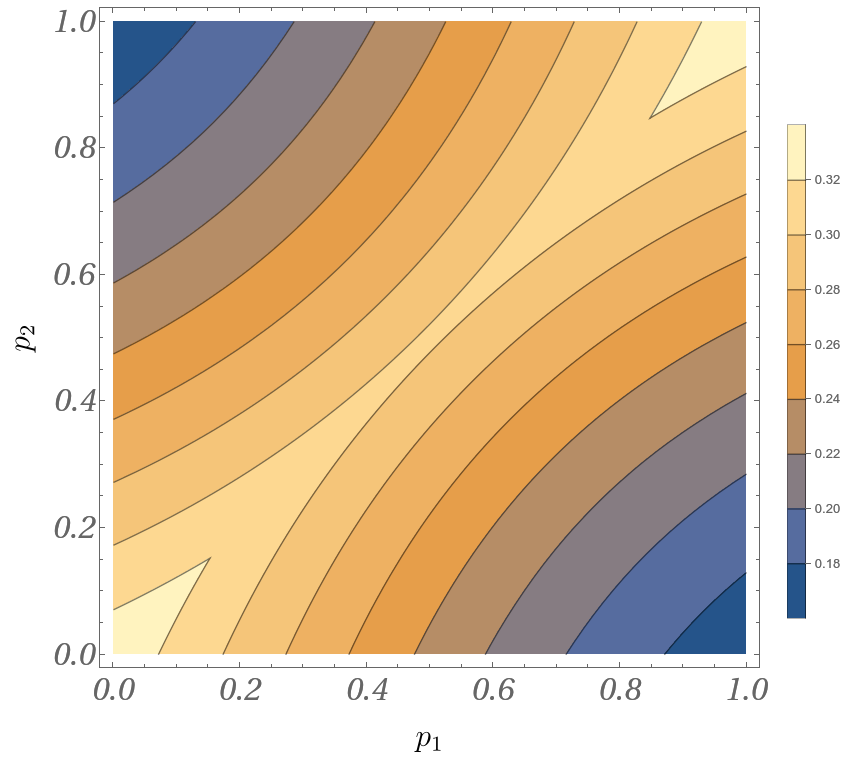
\includegraphics[width=12 cm]{img/F_1_4_CIEP.png}
    \caption{Contour plot of $F_1(p_1,p_2)$ for $N=4$.}
    \label{fig:F_1_4}
\end{figure}

\subsubsection{Special values of $F(.,.)$}

It is relatively easy to determine $F(1,1)$ i.e. the probability that the first row dominates all $i>2$ rows. For one column, $F_1(1,1)$ being:

\begin{equation}
    F_1(1,1) = \Pr(U_{1,1} > Z )
\end{equation}

Due to the independence of the columns:

\begin{equation}
    F(1,1) 
    =
    \left ( F_1(1,1) \right )^M
\end{equation}

Formally $F_1(1,1)$ can be expressed as:

\begin{equation}
    F_1(1,1) = 
    \int_{-\infty}^\infty \varphi(x) (\Phi(x))^{N-2} \ d x
\end{equation}

\begin{equation}
    F_1(1,1) = 
    \int_{-\infty}^\infty \Phi'(x) (\Phi(x))^{N-2} \ d x
\end{equation}

Substitution of variable to $p=\Phi(x)$ gives:

\begin{equation}
    F_1(1,1) = 
    \int_{0}^1 p^{N-2} \ d p
\end{equation}

\begin{equation}
    F_1(1,1) = 
    \frac{1}{N-1}
\end{equation}

\begin{equation}
    F(1,1) = 
    \frac{1}{(N-1)^M}
\end{equation}

By interchanging the first and second rows, we simply get:

\begin{equation}
    F(1,1) =  F(0,0)
\end{equation}

Therefore:

\begin{equation}
    F(1,1) =  F(0,0) = \frac{1}{(N-1)^M}
\end{equation}

We can continue by deriving an expression for $\Pr(E(p)) = F(p,p)$. To do this we first derive $\Pr(E_1(p)) = F_1(p,p)$.
Recalling that the sum of Gaussian random variables is Gaussian (and recalling that their variance adds up), we can write:

\begin{equation}
    F_1(p,p) = 
    \int_{-\infty}^\infty \varphi(x|0,p^2+q^2) (\Phi(x))^{N-2} \ d x
\end{equation}

\begin{equation}
    F_1(p,p) = 
    \int_{-\infty}^\infty \frac{1}{\sqrt{2 \pi} \sqrt{p^2+q^2}} e^{-\frac{1}{2}\frac{x^2}{p^2+q^2}} (\Phi(x))^{N-2} \ d x
\end{equation}

Due to the independence of columns:

\begin{equation}
    F(p,p) 
    =
    \left ( F_1(p,p) \right )^M
\end{equation}

Yielding the expression:

\begin{equation}
    F(p,p) = 
    \left ( 
    \int_{-\infty}^\infty \frac{1}{\sqrt{2 \pi} \sqrt{p^2+q^2}} e^{-\frac{1}{2}\frac{x^2}{p^2+q^2}} (\Phi(x))^{N-2} \ d x
    \right )^M
\end{equation}

\subsubsection{Derivative of $F(.,.)$}

To apply the formula \eqref{eq:PrE_Formula}, it is essential to determine the following derivative $f(p)$. To do this, first, we determine the derivative regarding $F_1(.,.)$:

\begin{equation}
    f_1(p)
    =
    \frac{\partial
    F_1(p - \varepsilon/2, p + \varepsilon/2) 
    }{\partial \varepsilon}
    \Bigg |_{\varepsilon=0_+}
\end{equation}

The derivative of $F(.,.)$ can be then determined simply by the chain rule:

\begin{equation}
    f(p)
    =
    \frac{\partial
    F(p - \varepsilon/2, p + \varepsilon/2) 
    }{\partial \varepsilon}
    \Bigg |_{\varepsilon=0_+}
    =
    M \  F_1(p,p)^{M-1} f_1(p)
\end{equation}

To proceed, we introduce the following boundary covariance matrix:

\begin{equation}
    \Sigma_\partial(p,\varepsilon)
    =
    \Sigma(p-\varepsilon/2,p+\varepsilon/2)
\end{equation}

Equation \eqref{eq:DetSigma} gives:

\begin{equation}
    \det(\Sigma_\partial(p,\varepsilon)) = \varepsilon^2
\end{equation}

Now, the inverse of the boundary covariance matrix looks the following:

\begin{equation}
    \Sigma_\partial(p,\varepsilon)^{-1} =
    \frac{1}{\varepsilon^2} 
    \begin{bmatrix}
    (p+\varepsilon/2)^2+(q-\varepsilon/2)^2 & -(p^2 + q^2) + \varepsilon^2/2 \\
    -(p^2 + q^2) + \varepsilon^2/2 & (p-\varepsilon/2)^2+(q+\varepsilon/2)^2
    \end{bmatrix}
\end{equation}

To calculate the first integral in the expression for $\eta(y|p_1,p_2)$ in eq. \eqref{eq:etaIntegral}, we make the substitution $x_1 \to y + a$, and rewrite the exponentiated term to the form on the right-hand side by finding the appropriate expressions for $c_1, \mu_1, \sigma_1$:

\begin{equation}
    -\frac{1}{2} (y+a,y) \Sigma_\partial(p,\varepsilon)^{-1} (y+a,y)^T = c_1(y|p,\varepsilon) - \frac{1}{2} \frac{(a-\mu_1(p,\varepsilon))^2}{\sigma_1(p,\varepsilon)^2} 
\end{equation}

Tedious but straightforward calculation gives that the appropriate expressions for the introduced variables are:

\begin{equation}
    \sigma_1(p,\varepsilon) = \frac{\varepsilon}{\sqrt{(p+\varepsilon/2)^2+(q-\varepsilon/2)^2}}
\end{equation}

\begin{equation}
    \mu_1(y|p,\varepsilon)
    =
    \frac{y \ \varepsilon (q-p-\varepsilon)}{(p+\varepsilon/2)^2+(q-\varepsilon/2)^2}
\end{equation}

\begin{equation}
    c_1(y|p,\varepsilon) = - \frac{1}{2} \frac{y^2}{(p+\varepsilon/2)^2+(q-\varepsilon/2)^2}
\end{equation}

We can treat the second part of the expression for $\eta(y|p_1,p_2)$ in the same manner. By making the substitution $x_2 \to y+b$ we get the analogous results:

\begin{equation}
    -\frac{1}{2} (y,y+b) \Sigma_\partial(p,\varepsilon)^{-1} (y,y+b)^T = c_2(y|p,\varepsilon) - \frac{1}{2} \frac{(b-\mu_2(p,\varepsilon))^2}{\sigma_2(p,\varepsilon)^2} 
\end{equation}

\begin{equation}
    \sigma_2(p,\varepsilon) = \frac{\varepsilon}{\sqrt{(p-\varepsilon/2)^2+(q+\varepsilon/2)^2}}
\end{equation}

\begin{equation}
    \mu_2(y|p,\varepsilon)
    =
    \frac{-y \ \varepsilon (q-p+\varepsilon)}{(p-\varepsilon/2)^2+(q+\varepsilon/2)^2}
\end{equation}

\begin{equation}
    c_2(y|p,\varepsilon) = - \frac{1}{2} \frac{y^2}{(p-\varepsilon/2)^2+(q+\varepsilon/2)^2}
\end{equation}

To determine the integrals, we will use the following general formula following from the expression for Gaussian distribution:

\begin{equation}
    \int_0^\infty e^{-\frac{(x-\mu)^2}{2 \sigma^2}} \ dx
    =
    \sqrt{2 \pi} \ \sigma \ \Phi \left( \frac{\mu}{\sigma} \right )
\end{equation}

After collecting the expressions and using the formula for the Gaussian integrals, we can define a new $\eta_\partial(y|p,\epsilon)$ variable on the boundary:

\begin{equation}
\begin{split}
    \eta_\partial(y|p,\varepsilon)
    = &
    \frac{1}{\sqrt{2 \pi}} \frac{e^{- \frac{1}{2} \frac{y^2}{(p+\varepsilon/2)^2+(q-\varepsilon/2)^2}}}{\sqrt{(p+\varepsilon/2)^2+(q-\varepsilon/2)^2}}
    \Phi \left( 
    \frac
    {
    y \ (q-p-\varepsilon)}
    {\sqrt{(p+\varepsilon/2)^2+(q-\varepsilon/2)^2}} 
    \right ) + \\
    &
    \frac{1}{\sqrt{2 \pi}} \frac{e^{- \frac{1}{2} \frac{y^2}{(p-\varepsilon/2)^2+(q+\varepsilon/2)^2}}}{\sqrt{(p-\varepsilon/2)^2+(q+\varepsilon/2)^2}}
    \Phi \left( 
    \frac
    {
    -
    y \ (q-p+\varepsilon)}
    {\sqrt{(p-\varepsilon/2)^2+(q+\varepsilon/2)^2}} 
    \right )
\end{split}
\end{equation}

Now we can take its Taylor-expansion with respect to $\varepsilon$ (assuming $\varepsilon>0$):

\begin{equation}
    \eta_\partial(y|p,\varepsilon)
    =
    \frac{e^{-\frac{1}{2} \frac{y^2}{p^2 + q^2}}}{\sqrt{2 \pi} \sqrt{p^2 + q^2}} +
    \varepsilon \ \eta_\partial'(y|p,0) + \mathcal{O}(\varepsilon^{-2})
\end{equation}

The explicit expression for $\eta_\partial'(y|p,0)$ looks the following:

\begin{equation}
\begin{split}
\eta_\partial'(y|p,0)
\left( -\frac{e^{-\frac{1}{2} \frac{y^2}{p^2 + q^2}}}{\sqrt{2 \pi} \sqrt{p^2 + q^2}} \right)^{-1}
= &
\frac{
    (p - q) (p^2 + q^2 - y^2) \left( \Phi\left( \frac{(q - p) y}{\sqrt{p^2 + q^2}} \right) -\Phi\left( \frac{(p - q) y}{\sqrt{p^2 + q^2}} \right) \right) 
}{
    2 (p^2 + q^2)^2
} + \\
&\frac{
    y \left( \Phi'\left( \frac{(q-p) y}{\sqrt{p^2 + q^2}} \right) + \Phi'\left( \frac{(p - q) y}{\sqrt{p^2 + q^2}} \right)  
    \right)
}{
    2 (p^2 + q^2)^{3/2}
    }
\end{split}
\end{equation}

Which can be simplified to:

\begin{equation}
\begin{split}
\eta_\partial'(y|p,0)
= &
 - \frac{e^{-\frac{1}{2} \frac{y^2}{p^2 + q^2}}}{\sqrt{2 \pi} \sqrt{p^2 + q^2}} \times \\
& \Bigg(
\frac{
    (p - q) (p^2 + q^2 - y^2) \left( \Phi\left( \frac{(q - p) y}{\sqrt{p^2 + q^2}} \right) -\Phi\left( \frac{(p - q) y}{\sqrt{p^2 + q^2}} \right) \right) 
}{
    2 (p^2 + q^2)^2
} + \\
&y \frac{
     e^{-\frac{1}{2} \frac{(q-p)^2 y^2}{p^2 + q^2}} 
}{
    \sqrt{2 \pi} (p^2 + q^2)^{3/2}
    }
    \Bigg)
\end{split}
\end{equation}

By which we can express $f_1(p)$ as:

\begin{equation}
    f_1(p)
    =
    \int_{-\infty}^\infty \eta_\partial'(y|p,0) \  (\Phi(y))^{N-2} \ d y
\end{equation}

\subsubsection{General $N$, $M$ case}

To calculate $\Pr(E)$ we can now give an integral formula for the general $N$, $M$ case:

\begin{equation}
    \Pr(E) 
    = 
    \frac{1}{(N-1)^M}
    - M \int_0^1
    F_1(p,p)^{M-1} f_1(p)
    \ d p
\end{equation}

Numerical results can be obtained by collecting the terms and performing the numerical integrals. To give concrete examples we collected numerical results for $N \in \{3,\dots,7\}$ and $M \in \{1,\dots,5\}$ cases and presented them in the following table:

\begin{table}[H]
\centering
\begin{tabular}{|c|c|c|c|c|c|}
\hline
$N \backslash M$ & 1 & 2 & 3 & 4 & 5 \\ \hline
3 & 0.666667 & 0.416667 & 0.250000 & 0.145833 & 0.083333 \\ \hline
4 & 0.500000 & 0.215792 & 0.086387 & 0.033042 & 0.012259 \\ \hline
5 & 0.400000 & 0.128927 & 0.037767 & 0.010491 & 0.002819 \\ \hline
6 & 0.333333 & 0.084715 & 0.019340 & 0.004178 & 0.000874 \\ \hline
7 & 0.285714 & 0.059513 & 0.011067 & 0.001949 & 0.000334 \\ \hline
\end{tabular}
\caption{Numerical values of $\Pr(E)$ as a function of $N$ and $M$}
\end{table}

\subsubsection{Special case, $N=3$}

In general, the solution seems to be computable numerically only; however, for $N=3$ (and $M=1$), there is a closed-form solution.
We introduce the following integral:

\begin{equation}
    I_\partial = M \int_0^1 F_1(p,p)^{M-1} f_1(p) \ dp
\end{equation}

We can get by simple argumentation (for two Gaussians with the same mean, it is equally probable that the first or the second is greater) or by direct calculation that for $N=3$, $\forall p \in [0,1]$:

\begin{equation}
    F_1(p,p) = 1/2
\end{equation}

Remarkably, the integral of $\eta_\partial'(y|p,0)$ with respect to $p$ can be evaluated explicitly (this can be checked by taking the derivative):

\begin{equation}
\int \eta_\partial'(y|p,0) \ dp
=
-\frac{e^{-\frac{y^2}{2 (p^2 + q^2)}} \left( \Phi\left( \frac{(p - q) y}{\sqrt{p^2 + q^2}} \right) - \frac{1}{2} \right)}{\sqrt{p^2 + q^2} \sqrt{2 \pi}}
\end{equation}

Yielding the following result for the definite integral:

\begin{equation}
\int_0^1 \eta_B'(y|p,0) \ dp
=
- \frac{1}{\sqrt{2 \pi}} e^{-\frac{y^2}{2}}
\left(
2 \ \Phi(y) - 1
\right)
\end{equation}

Therefore, for $N=3$:

\begin{equation}
    I_\partial = M \int_0^1 (1/2)^{M-1} f_1(p) \ dp
\end{equation}

After recalling the expression for $f_1(p)$ we get:

\begin{equation}
    I_\partial = \frac{M}{2^{M-1}} \int_0^1 
    \int_{-\infty}^\infty \eta_B'(y|p,0) \  (\Phi(y))^{N-2} 
    \ d y
    \ dp
\end{equation}

After interchanging the integrals, we get:

\begin{equation}
    I_\partial = \frac{M}{2^{M-1}}
    \int_{-\infty}^\infty 
    - \frac{1}{\sqrt{2 \pi}} e^{-\frac{y^2}{2}}
\left(
2 \ \Phi(y) - 1
\right)
    \  \Phi(y)
    \ d y
\end{equation}

Which can be calculated by substituting $y \to \Phi(y)$, giving:

\begin{equation}
    I_\partial = -\frac{M}{2^{M-1}}
\left(
2 \ \frac{1}{3} - \frac{1}{2}
\right)
=
 -\frac{M}{2^{M-1}} \ \frac{1}{6}
\end{equation}


Recalling the expression for $\Pr(E)$:

\begin{equation}
    \Pr(E) 
    = 
    \frac{1}{(N-1)^M}
    - I_\partial
\end{equation}

For $N=3$

\begin{equation}
    \Pr(E) 
    = 
    \frac{1}{2^M}
    +
    \frac{M}{2^{M-1}} \ \frac{1}{6}
    =
    \frac{6 + 2 \ M}{6 \ 2^M}
\end{equation}

Resulting in the following explicit expression:

\begin{equation}
\boxed{
    \Pr(E) 
    = 
    \frac{3 + M}{3 \ 2^M}
    =
    \frac{1}{2^M} 
    \left(
    1 + \frac{M}{3}
    \right),
    \quad \text{for } N=3
    }
\end{equation}

\subsubsection{Special case, $M=1$}

When $M=1$, then the integral $I_\partial$ becomes simply:

\begin{equation}
    I_\partial = \int_0^1 f_1(p) \ dp
\end{equation}

Which can be simplified to:

\begin{equation}
    I_\partial = 
    \int_{-\infty}^\infty 
    - \frac{1}{\sqrt{2 \pi}} e^{-\frac{y^2}{2}}
\left(
2 \ \Phi(y) - 1
\right)
    \  \Phi(y)^{N-2}
    \ d y
\end{equation}

Using the substitution $y \to \Phi(y)$, we get:

\begin{equation}
    I_\partial = 
    -
    \left(
    2 \frac{1}{N} - \frac{1}{N-1}
    \right)
\end{equation}

Therefore for $M=1$:

\begin{equation}
    \Pr(E) 
    = 
    \frac{1}{N-1}
    - I_\partial
    =
    \frac{1}{N-1} + 2 \frac{1}{N} - \frac{1}{N-1}
\end{equation}

\begin{equation}
\boxed{
    \Pr(E) 
    = 
    \frac{2}{N}, \quad \text{for } M=1
    }
\end{equation}

\section{Summary}

\paragraph{Conjecture, integral formula and numerical results:}
In this paper, we conjectured a general formula termed  ``continuous
inclusion-exclusion principle'' and used it to calculate a nontrivial result.
The problem we aimed to solve is to calculate the probability of a random Gaussian utility matrix being dominated by some mixture of its first two rows.
We -- assuming the conjecture to be true -- derived a general integral formula for $N\times M$ random matrices, calculated its numerical value for $N \in \{3,\dots,7\}, M \in \{1,\dots,5\}$ cases and gave exact formulas for $N=3, M \in \mathbb{N}$ and $N \in \mathbb{N}, M=1$ edge cases.

\paragraph{Checking the results with alternative methods:}
To check the feasibility of the results in Appendix B, we report the results of Monte Carlo simulations, which are inline (do not differ significantly) from the numerical values obtained by the conjectured integral formula.
In Appendix D, we gave an exact derivation of the probabilities of domination for the $N=3, M \in \mathbb{N}$ edge case, which matches the results obtained by the conjectured integral formula. In Appendix D, we calculated the probability for $M=1$, which also matched the conjectured results.

\paragraph{Example and counterexample for the conjecture:}
To put the ``continuous inclusion-exclusion principle'' into perspective, in Appendix A, we showed a simple toy example, when every part of the formula can be determined and where it gives the correct result. To emphasize the need to find criteria for when the method could be used, we showed a trivial counterexample when the method broke down.

\subsection{Future work}

\paragraph{Proving the conjecture:}
In my view, the paper gives a strong motivation to explore further the conjectured ``continuous inclusion-exclusion principle''. Still, naturally, against all results and numerical sanity checks, the general formula remained unproven.
To make a rigorous proof, a discretization of the continuous $p\in [0,1]$ space and then the usage of a multi-dimensional Euler-Maclaurin formula \cite{aper:MultyDimEylerMaclaurin01,paper:MultyDimEylerMaclaurin02}  seems a natural approach. However, this further exploration remains the subject of another paper.

\paragraph{Generalization for three or more dominating rows:}
It seems conceivable that similar integral formulas are derivable for the probability of the domination of the first three rows. However, the calculation becomes much more complicated because we can not simply use the simplification of multiple intersections. What remains a possibility is a ``convex expansion'' of dominating regions. In this approach, only convex regions with converging to $0$ volume will give contributions in the $L\to \infty$ limit, opening the possibility to obtain an integral formula, but the necessary derivation seems much more complicated than the derivation presented in this paper.
The details of such a formula remain in the realm of future works.


\begin{appendices}

\section{Example and counterexample}

At this point, the "continuous inclusion-exclusion principle" is a heuristic that seems to work in some cases but fails in others.
This section shows an example and a counter-example to demonstrate both scenarios.

\subsection{Example: length of an interval}

Maybe the simplest example to demonstrate the successful application of the ``continuous inclusion-exclusion principle'' heuristics is to determine the length of an interval, which has been defined as the union of shifted intervals with unit length.

$E(\alpha)$ being a unit interval $[0,1] \subset \mathbb{R}$ shifted to the right by $\alpha$: 

\begin{equation}
    E(\alpha) = [\alpha, 1 + \alpha]
\end{equation}

Now we can define a set $E$ -- being itself an interval -- as a continuum union of shifted intervals:

\begin{equation}
    E = \bigcup_{\alpha \in [0,1]} E(\alpha)
\end{equation}

It is easy to determine $E$ and its length ($\mu(E)$) explicitly:

\begin{equation}
    E = [0,2] \implies \boxed{\mu(E) = 2}
\end{equation}

Now, let's check if the application of the ``continuous inclusion-exclusion principle'' formula gives the same result.
First, we spell out the formula:

\begin{equation}
    \mu(E) = \lim_{L \to \infty} \sum_{n=1}^\infty (-1)^{n-1} L^n
    \underset{0 \le \alpha_1 < \dots < \alpha_n \le 1}{\int\dots\int}
    \mu \left ( 
    \bigcap_{k=1}^n E(\alpha_k)
    \right ) 
    d\alpha_1\dots d\alpha_n
\end{equation}

If $\alpha_1 < \alpha_2 < \dots < \alpha_n$, then the length of the intersections of $E(\alpha_i)$ is determined only by the smallest and the largest $\alpha_i$, i.e. $\alpha_1$ and $\alpha_n$:

\begin{equation}
    \mu \left ( 
    \bigcap_{k=1}^n E(\alpha_k)
    \right ) 
    =
    \mu \left (
    E(\alpha_1) \cap E(\alpha_n)
    \right )
    =
    F(\alpha_1,\alpha_n)
    =1+\alpha_1-\alpha_n
\end{equation}

or 

\begin{equation}
    F(\alpha_1,\alpha_n)
    =1-(\alpha_n-\alpha_1)
\end{equation}


Therefore, for all $n\ge 2$

\begin{equation}
    \underset{0 \le \alpha_1 < \dots < \alpha_n \le 1}{\int\dots\int}
    \mu \left ( 
    \bigcap_{k=1}^n E(\alpha_k)
    \right ) 
    d\alpha_1\dots d\alpha_n
    =
    \iint\limits_{0 \le \alpha_1 < \alpha_n \le 1}
    \frac{(\alpha_n-\alpha_1)^{n-2}}{(n-2)!}
    (1-(\alpha_n-\alpha_1)) \ d\alpha_1 d\alpha_n
\end{equation}

In this case, we can explicitly calculate all terms. By applying the substitution $\alpha_n-\alpha_1 \to \Delta, \alpha_n \to \alpha_n$ we can determine the value of the following integral:

\begin{equation}
    \iint\limits_{0 \le \alpha_1 < \alpha_n \le 1}
    (\alpha_n-\alpha_1)^{n-2}
    \ d\alpha_1 d\alpha_n
    =
    \int_0^1 \int_0^{\alpha_n} \Delta^{n-2} \ d \Delta d \alpha_n
\end{equation}

\begin{equation}
    \int_0^1 \int_0^{\alpha_n} \Delta^{n-2} \ d \Delta d \alpha_n
    =
    \frac{1}{n-1} \int_0^1  \alpha_n^{n-1} \ d \alpha_n
    =
    \frac{1}{n(n-1)}
\end{equation}

Applying the previous result, we get:

\begin{equation}
    \iint\limits_{0 \le \alpha_1 < \alpha_n \le 1}
    (\alpha_n-\alpha_1)^{n-2}
    (1-(\alpha_n-\alpha_1)) \ d\alpha_1 d\alpha_n
    =
    \frac{1}{n(n-1)} - \frac{1}{(n+1)n}
\end{equation}

After simplifying the terms, we get the following:

\begin{equation}
    \frac{1}{n(n-1)} - \frac{1}{(n+1)n} = \frac{2}{(n-1)n(n+1)}
\end{equation}

Therefore:

\begin{equation}
    \iint\limits_{0 \le \alpha_1 < \alpha_n \le 1}
    \frac{(\alpha_n-\alpha_1)^{n-2}}{(n-2)!}
    (1-(\alpha_n-\alpha_1)) \ d\alpha_1 d\alpha_n
    =
    \frac{2}{(n+1)!}
\end{equation}

For $n=1$, we have:

\begin{equation}
    \int_0^1 \mu(E_\alpha) \ d \alpha = 1 = \frac{2}{(1+1)!}
\end{equation}

Now we can explicitly determine the $L$-dependent infinite sum $G(L)$, appearing in the formula:

\begin{equation}
    G(L) = \sum_{n=1}^\infty (-1)^{n-1} L^n
    \frac{2}{(n+1)!}
\end{equation}

This we can explicitly calculate:

\begin{equation}
    G(L)
    =
    \frac{2}{L} \sum_{n=1}^\infty (-1)^{n+1} L^{n+1}
    \frac{1}{(n+1)!}
\end{equation}

\begin{equation}
    G(L)
    =
    \frac{2}{L} \sum_{n'=2}^\infty \frac{1}{n'!} (-L)^{n'}
\end{equation}

\begin{equation}
    G(L)
    =
    \frac{2}{L} 
    \left(
    e^{-L} - (1-L)
    \right)
\end{equation}

\begin{equation}
     G(L)
    =
    2 - \frac{2}{L} + \frac{2}{L} e^{-L}
\end{equation}

After having this explicit formula for $G(L)$ we can take its $L \to \infty$ limit to get $\mu(E)$:

\begin{equation}
    \mu(E) = \lim_{L \to \infty} 
    G(L)
\end{equation}

\begin{equation}
\boxed{
    \mu(E) = \lim_{L \to \infty} 
    \left(
    2 - \frac{2}{L} + \frac{2}{L} e^{-L}
    \right)
    =
    2
    }
\end{equation}

\paragraph{Checking the integral formula:}
In this simple case, we can check the integral formula derived by exploiting the simplification for $n>2$ intersections and exchanging summation with integration:

\begin{equation}
    \mu(E) 
    = 
    \frac{1}{2} \left ( F(0,0)+F(1,1) \right ) 
    - \int_0^1
    \frac{\partial
    F(p - \Delta/2, p + \Delta/2) 
    }{\partial \Delta}
    \Bigg |_{\Delta=0_+}
    \ dp
\end{equation}

For $F(.,.)$ we have:

\begin{equation}
    F(0,0)=F(1,1)=1
\end{equation}

\begin{equation}
    F(p - \Delta/2, p + \Delta/2)
    =
    1-\Delta
\end{equation}

Therefore:

\begin{equation}
\boxed{
    \Pr(E) 
    = 
    \frac{1}{2} \left ( 1 + 1 \right ) 
    - \int_0^1
    (-1)
    \ dp
    =
    2
    }
\end{equation}

\subsection{Counterexample: interval from points}

We can construct a very straightforward counterexample by defining an interval as the continuum union of single points:

\begin{equation}
    E(\alpha) = [\alpha, \alpha] = \{\alpha\}
\end{equation}

\begin{equation}
    E = \bigcup_{\alpha \in [0,2]} E(\alpha)
\end{equation}

Naturally, we have:

\begin{equation}
    E = [0,2] \implies \mu(E) = 2
\end{equation}

However, for all $E(\alpha)$ we have:

\begin{equation}
    \mu(E(\alpha)) = 0
\end{equation}

Therefore, for any finite $n$:

\begin{equation}
    \mu \left ( 
    \bigcap_{k=1}^n E(\alpha_k)
    \right ) 
    =
    \mu \left (
    E(\alpha_1) \cap E(\alpha_n)
    \right )
    =
    F(\alpha_1,\alpha_n)
    =0
\end{equation}

Therefore, both explicit calculation and the integral formula can give only $0$:

\begin{equation}
    \mu(E) \ne \lim_{L \to \infty} \sum_{n=1}^\infty (-1)^{n-1} L^n
    \underset{0 \le \alpha_1 < \dots < \alpha_n \le 1}{\int\dots\int}
    \mu \left ( 
    \bigcap_{k=1}^n E(\alpha_k)
    \right ) 
    d\alpha_1\dots d\alpha_n
\end{equation}

\begin{equation}
    \mu(E) 
    \ne
    \frac{1}{2} \left ( F(0,0)+F(1,1) \right ) 
    - \int_0^1
    \frac{\partial
    F(p - \Delta/2, p + \Delta/2) 
    }{\partial \Delta}
    \Bigg |_{\Delta=0_+}
    \ dp
\end{equation}

Because:

\begin{equation}
    2 \ne 0
\end{equation}

\section{Numerical evidence}

To check the numerical results, we performed Monte Carlo simulations \cite{book:MonteCarlo} to compare the numerically calculated theoretical probabilities with the simulated empirical frequencies.

The algorithm checking the dominance of the first two rows can be summarized as follows:
Determine for every column the interval $I_i$, which contains all $p_i$ values, for which the mixture of first and second rows dominate the rest (in the $i$-th column).
If $X$ and $Y$ are the value of the first and second row respectively (in the $i$-th column) and $Z$ is the maximum of the remaining rows, then the critical $p$ which is the lower or upper limit of $I_i$ can be calculated as: 

\begin{equation}
    p \ X + (1-p) Y = Z \implies p = \frac{Y-Z}{Y-X}
\end{equation}

(If $X<Z<Y$, then $I=[0,p]$, and if $Y<Z<X$ then $I=[p,1]$)

To determine if there exists a mixing ratio $p$ for which the mixture of the first and second rows dominates all the rows, we can simply take the intersection of all $I_i$ intervals and see if it is empty. If it is not empty, then there is a mixture by which domination can be achieved.

The following algorithm is a more efficient implementation of the above-described principle:

\begin{algorithm}[H]
\caption{Dominance Check of Two Rows in a Random Matrix}
\begin{algorithmic}[1]
\State \textbf{Input:} Number of columns $M$, Number of rows $N$
\State \textbf{Output:} True or False indicating dominance

\State Low $\gets 0$
\State High $\gets 1$

\For{$j \gets 1$ to $M$}
    \State Generate $X \sim \mathcal{N}(0, 1)$
    \State Generate $Y \sim \mathcal{N}(0, 1)$
    \State Generate $Z$ as the maximum of $N-2$ independent Gaussian random variables $\{Z_1, Z_2, \ldots, Z_{N-2}\}$, where $Z_i \sim \mathcal{N}(0, 1)$
    
    \If{$X \leq Z$ \textbf{and} $Y \leq Z$}
        \State \Return False
    \Else
        \If {Not $(X > Z$ \textbf{and} $Y > Z)$}
            \If{$X > Y$}
                \State Low $\gets \max($Low$, \frac{Z - Y}{X - Y})$
            \ElsIf{$X < Y$}
                \State High $\gets \min($High$, \frac{Y - Z}{Y - X})$
            \EndIf
            \If{Low $>$ High}
                \State \Return False
            \EndIf
        \EndIf
    \EndIf
\EndFor

\State \Return True
\end{algorithmic}
\end{algorithm}

Results based on implementing the algorithm in {\it Wolfram Mathematica} are collected in the table below:

\begin{table}[H]
\centering
\begin{tabular}{|c|c|c|c|c|c|}
\hline
$N \backslash M$ & 1 & 2 & 3 & 4 & 5 \\ \hline
3 & 667087 & 416483 & 249532 & 145620 & 83738 \\ \hline
4 & 499816 & 216128 & 86103 & 32972 & 12135 \\ \hline
5 & 399810 & 128832 & 37695 & 10443 & 2721 \\ \hline
6 & 333536 & 84898 & 19160 & 4192 & 831 \\ \hline
7 & 285218 & 59791 & 11059 & 1925 & 342 \\ \hline
\end{tabular}
\caption{Monte Carlo simulation results after one million runs for different $N, M$ values.}
\end{table}

These results can be compared to the values obtained by numerical integration.
To compare theoretical and empirical results, we calculated the ``Z-scores'' (related to ``Z test'' \cite{book:StatisticsIntro}) of the measured quantities, assuming that the random counts have a Binomial distribution with a parameter equal to the theoretical value:

\begin{equation}
    z = \frac{n/K-p_T}{\sqrt{p_T(1-p_T)/K}}
\end{equation}

Where $K=1000000=10^6$ is the total number of runs, $n$ is the count of seeing event $E$, while $p_T$ is the theoretical probability for event $E$.

\begin{table}[H]
\centering
\begin{tabular}{|c|c|c|c|c|c|}
\hline
$N \backslash M$ & 1 & 2 & 3 & 4 & 5 \\ \hline
3 & -0.89 & 0.37 & 1.08 & 0.60 & -1.46 \\ \hline
4 & 0.37 & -0.82 & 1.01 & 0.39 & 1.13 \\ \hline
5 & 0.39 & 0.28 & 0.38 & 0.47 & 1.85 \\ \hline
6 & -0.43 & -0.66 & 1.31 & -0.21 & 1.46 \\ \hline
\end{tabular}
\caption{``Z-scores'' for different $N, M$ values}
\end{table}

Based on the obtained ``Z-values'', we can say that the empirical results do not deviate significantly ($95\%$) from the theoretical values.

\subsection{Modified Box-Muller transform}

In the \texttt{C} implementation of the described algorithm, the following modified Box-Muller algorithm made the program $\approx 2$-times more effective:

\begin{algorithm}[H]
\caption{Modified Box-Muller Transform to Generate the Maximum of Two Gaussian Random Variables}
\begin{algorithmic}[1]
\State \textbf{Input:} No input required
\State \textbf{Output:} $\max(X,Y)$,  $X, Y \sim \mathcal{N}(0, 1)$

\State Generate $U_1 \sim \mathcal{U}(0, 1)$
\State Generate $U_2 \sim \mathcal{U}(0, 1)$

\State $X \gets \sqrt{-2 \log(U_1)} \sin(\pi \ (U_2 + 1/4))$
\State \Return $X$
\end{algorithmic}
\end{algorithm}

\section{Exact calculation for the $N=3, M=2$ case}

Here we present an explicit and exact calculation for the probability $\Pr(E)$ for three rows ($N=3$) and two columns ($M=2$).
To tackle this question, first, we can take random variables in the first column:

\begin{equation}
    X = U_{1,1}, \quad Y = U_{2,1}, \quad Z = U_{3,1}
\end{equation}

A constant shift in all utilities does not change the interval $I$, which contains the mixing ratios resulting in a mixture of the first and second rows that is greater than the third row.
This can be seen from the formula for the critical value of $p$:

\begin{equation}
    p = \frac{Y-Z}{Y-X}  = \frac{(Y-C)-(Z-C)}{(Y-C)-(X-C)}
\end{equation}

By choosing $C=Z$, we can introduce the following reduced random variables:

\begin{equation}
    X' = X - Z, \quad Y'=Y - Z
\end{equation}

$X'$ and $Y'$ are correlated Gaussian random variables. However we can find new $(V,W)$ variables which are independent, and are standard Gaussians $V,W \sim \mathcal{N}(0,1)$:


\begin{equation}
    V = \frac{1}{\sqrt{6}}(X + Y - 2 Z), \quad
    W = \frac{1}{\sqrt{2}} (X - Y)
\end{equation}

\begin{equation}
    X' = \frac{\sqrt{3}}{\sqrt{2}} V + \frac{1}{\sqrt{2}} W, \quad
    Y' = \frac{\sqrt{3}}{\sqrt{2}} V - \frac{1}{\sqrt{2}} W
\end{equation}

One can easily check that:

\begin{equation}
    \mathbb{E}[V^2] = \frac{1}{6} (1 + 1 + 2^2) = 1
\end{equation}

\begin{equation}
    \mathbb{E}[W^2] = \frac{1}{2} (1 + 1) = 1
\end{equation}

\begin{equation}
    \mathbb{E}[V \ W] = \frac{1}{12} ( \mathbb{E}[(X-Z)^2] - \mathbb{E}[(Y-Z)^2] ) = 0
\end{equation}

Therefore, $V$ and $W$ are indeed standard, independent Gaussian random variables.

Concerning domination, i.e. events $E(p)$ we can distinguish four regions defined by $X',Y'$ variables:

\begin{equation}
\begin{split}
    \mathcal{D}_{--}: X' < 0, Y' < 0; & \quad
    \mathcal{D}_{-+}: X' < 0, Y' > 0; \\
    \mathcal{D}_{+-}: X' > 0, Y' < 0;  & \quad
    \mathcal{D}_{++}: X' > 0, Y' > 0. 
\end{split}
\end{equation}

\begin{itemize}
    \item If the values happen to fall into $\mathcal{D}_{--}$, then there is no mixture which can dominate, i.e. $I_{--}=\emptyset$.
    \item If the values happen to fall into $\mathcal{D}_{+-}$, then the first row dominates, while the second does not, i.e. $\exists p\in [0,1]$ that $I_{+-}=[p,1]$.
    \item If the values happen to fall into $\mathcal{D}_{-+}$, then the second row dominates, while the first does not, i.e. $\exists p\in [0,1]$ that $I_{-+}=[0,p]$.
    \item If the values happen to fall into $\mathcal{D}_{++}$, then all mixtures dominate, i.e. $I_{++}=[0,1]$.
\end{itemize}

Let us see how these domains look on the $(V, W)$ plain:

\begin{figure}[H]
    \centering
    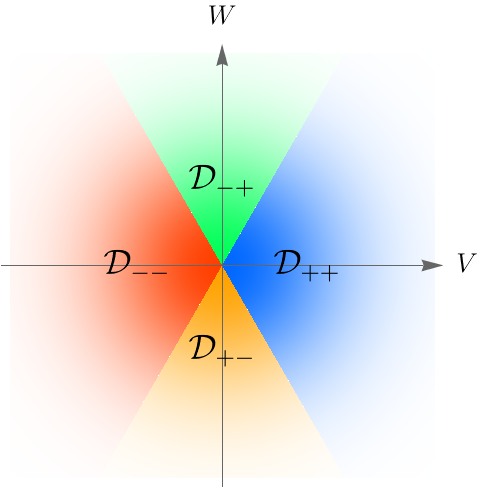
\includegraphics[width=8 cm]{img/VW_regions.png}
    \caption{$\mathcal{D}_{--}, \mathcal{D}_{-+}, \mathcal{D}_{+-}, \mathcal{D}_{++}$ regions on the $(V,W)$ plain.}
    \label{fig:VW_D}
\end{figure}

It is straightforward to determine the boundaries of the regions:

\begin{equation}
    X' = 0 \implies \frac{\sqrt{3}}{2} V + \frac{1}{2} W = 0
\end{equation}

\begin{equation}
    Y' = 0 \implies \frac{\sqrt{3}}{2} V - \frac{1}{2} W = 0
\end{equation}

Therefore, on the $(V, W)$ plain, these four regions are the regions separated by two lines, which cross the origin and are tilted from $V$ axes by $\pm \theta$ angle:

\begin{equation}
    \theta = \pi/3
\end{equation}

The distribution is a standard uncorrelated two-dimensional Gaussian on the $(V, W)$ plain. Therefore, it has rotational symmetry in 2D.
This makes calculating the probabilities of these regions very easy; we only need to determine the sector angle for each and divide it by $2 \pi$:


\begin{equation}
    \Pr((X',Y') \in \mathcal{D}_{--}) = \frac{2 \theta}{2 \pi} = 1/3
\end{equation}

\begin{equation}
    \Pr((X',Y') \in \mathcal{D}_{++}) = \frac{2 \theta}{2 \pi} = 1/3
\end{equation}

\begin{equation}
    \Pr((X',Y') \in \mathcal{D}_{+-}) = \frac{\theta}{2 \pi} = 1/6
\end{equation}

\begin{equation}
    \Pr((X',Y') \in \mathcal{D}_{-+}) = \frac{\theta}{2 \pi} = 1/6
\end{equation}

In $\mathcal{D}_{+-}$ the mixing ratio can be in the interval $I_{+-} = [p,1]$, while in $\mathcal{D}_{-+}$ in the interval $I_{-+} = [0,p]$.
We recall the following formula to determine $p$:

\begin{equation}
    p = \frac{Y-Z}{Y-X} = \frac{-Y'}{X'-Y'}
\end{equation}

and so:

\begin{equation}
    1-p =  \frac{X'}{X'-Y'}
\end{equation}

We can introduce the random angle $\Phi$ on the $(V,W)$ plain, which measures the inclination from the $W$ axes: 

\begin{equation}
    \Phi = - \arctan(V/W) =
    \arctan\left( -\frac{1}{\sqrt{3}} \frac{X'+Y'}{X'-Y'} \right)
\end{equation}

The distribution on the $(V,W)$ plain has a rotational symmetry, therefore
if $(X',Y') \in \mathcal{D}_{-+} \cup \mathcal{D}_{+-}$ then:

\begin{equation}
    \Phi_{\pm},\Phi_{\mp} \sim \mathcal{U}(-\pi/6,\pi/6)
\end{equation}

There is a one to one map $\phi : [0,1] \mapsto [-\pi/6,\pi/6]$ between this angle and the critical mixing ratio $p$:

\begin{equation}
    \phi(p) = \arctan \left( \frac{1}{\sqrt{3}} (2 p-1) \right)
\end{equation}

This is a monotonic function, therefore order-preserving:

\begin{equation}
    p_1 > p_2  \iff \phi(p_1) > \phi(p_2)
\end{equation}


\subsubsection{$M=2$}

For $M=2$, there are $4 \times 4 = 16$ possibilities to consider because both the first and the second row can fall to the four $\mathcal{D}_{s_1,s_2}$ ($s_i \in \{+,-\}$) domain independently.

\begin{itemize}
    \item If any columns fall to $\mathcal{D}_{--}$, then there can not be a dominating ratio i.e. $E$ is not occurring.
    \item In the remaining possibilities, only those situations do not result in domination, in which the first row falls to $\mathcal{D}_{-+}$ and the other $\mathcal{D}_{+-}$ or vice versa.
    \begin{itemize}
        \item In the $\mathcal{D}_{-+}$, $\mathcal{D}_{+-}$ case the first column has a $I_1 = [0,p_1]$ interval, while the second column $I_2=[p_2,1]$.
        For domination, the intersection of the intervals has to be non-empty, i.e. $p_1>p_2$.
        This is equivalent to the requirement: $\Phi_{\mp,1} > \Phi_{\pm,2}$.
        From the uniform and independent distribution of both angular random variables, it follows that $\Pr(\Phi_{\mp,1} > \Phi_{\pm,2}) = 1/2$.
    \end{itemize}
\end{itemize}

We can collect the conditional probabilities of dominance $P(.,.)$ depending on values falling to the $4 \times 4$ domains:

\begin{equation}
    P(\mathcal{D}_I,\mathcal{D}_J) 
    =
    \Pr(E \ | \ (X'_1,Y'_1) \in \mathcal{D}_I \wedge (X'_2,Y'_2) \in \mathcal{D}_J \}
\end{equation}

\begin{table}[H]
\begin{center}
\begin{tabular}{c | c | c c c c} 
 Domain &   & $\mathcal{D}_{++}$ & $\mathcal{D}_{-+}$ & $\mathcal{D}_{+-}$ & $\mathcal{D}_{--}$ \\
 \hline
   & $\Pr$ & 1/3 & 1/6 & 1/6 & 1/3 \\ 
 \hline
 $\mathcal{D}_{++}$ & 1/3 & 1 & 1 & 1 & 0 \\
 $\mathcal{D}_{-+}$ & 1/6 & 1 & 1 & 1/2 & 0 \\
 $\mathcal{D}_{+-}$ & 1/6 & 1 & 1/2 & 1 & 0 \\
 $\mathcal{D}_{--}$ & 1/3 & 0 & 0 & 0 & 0 \\
\end{tabular}
\end{center}
\caption{Conditional probabilities of dominance $P(.,.)$ and probabilities of falling to specific domains $\Pr(\mathcal{D}_I), \Pr(\mathcal{D}_J)$.}
\end{table}

To get the probability of dominance, we simply need to take the weighted sum of conditional probabilities:

\begin{equation}
    \Pr(E)
    =
    \sum_{I,J} 
    P(\mathcal{D}_I,\mathcal{D}_J)
    \Pr(\mathcal{D}_I)
    \Pr(\mathcal{D}_J)
\end{equation}

Which can be calculated as:

\begin{equation}
    \Pr(E)
    =
    \left(\frac{2}{3}\right)^2 - \left(\frac{1}{6}\right)^2 = \frac{16-1}{36} = \frac{15}{36}
\end{equation}

Resulting in the exact value:

\begin{equation}
    \boxed{
    \Pr(E)
    =
    \frac{5}{12}, \quad \text{for } N=3, M=2
    }
\end{equation}

\section{$N=3$, $M\in\mathbb{N}$}

Building on the notation and results in the previous section, we can generalize the results to any $M \in \mathbb{N}$ columns.
To make the calculation simpler, we can introduce a simple transformation, which maps the angular random variable $\Phi$ to a ratio $R$ having a standard uniform distribution:

\begin{equation}
    R = \frac{\Phi+\pi/6}{\pi/3}
\end{equation}

\begin{equation}
    R \sim \mathcal{U}(0,1)
\end{equation}

For further use, we calculate the probability of:

\begin{equation}
    f_P(j,k) 
    =
    \Pr(\min(R_1,\dots,R_j)>\max(R'_1,\dots,R'_k))
\end{equation}

Where $R_a,R'_b \sim \mathcal{U}(0,1)$.

It is easy to determine the cumulative distribution function of $\max(R'_1,\dots,R'_k)$, from which the density function can be derived:

\begin{equation}
    F_{\max}(r) = r^k
    \implies
    f_{\max} = k \ r^{k-1}
\end{equation}

Alternatively, for the minimum, we get:

\begin{equation}
    F_{\min}(r) = 1 - (1-r)^j
    \implies
    f_{\min} = j \ (1-r)^{j-1}
\end{equation}

With these density functions $f_P(j,k)$ can be defined as an integral:

\begin{equation}
    f_P(j,k) = 
    \underset{1 \ge r_1 > r_2 \ge 0}{\iint}
    (j \ (1-r_1)^{j-1})(k \ r_2^{k-1})
    \ dr_1 dr_2
\end{equation}

Which can be determined explicitly, resulting:

\begin{equation}
    f_P(j,k) = 
    \frac{j! k!}{(j+k)!}
\end{equation}

For general $M \in \mathbb{N}$ columns, there will be $4^M$ possible configurations of domains.
However, what really matters is how many columns fall to each $\mathcal{D}_I$ domain.
Assuming that $i$ number of columns fall into $\mathcal{D}_{++}$, $j$ number of columns into $\mathcal{D}_{-+}$, $k$ into $\mathcal{D}_{+-}$ and $\ell$ into $\mathcal{D}_{--}$ we can make the following observations:

\begin{itemize}
    \item If any columns fall to $\mathcal{D}_{--}$, i.e. $\ell > 0$, then the first two rows can not dominate the third one.
    \item If $\ell=0$ then the only excluding criteria for dominance is when both $j,k>0$, and the intersection of $I_{+-}$ and $I_{-+}$ domains are empty.
    \begin{itemize}
        \item To calculate the conditional probability of dominance, given that there are $j$ columns in $\mathcal{D}_{-+}$ and $k$ columns in $\mathcal{D}_{+-}$ we can first determine the distribution for the ratio interval $I^R_{-+}(j) = \cap_{\iota=1}^j I^R_{-+,\iota} = [0, R_{-+}(j)]$,
        and $I^R_{+-}(k) = \cap_{\iota=1}^k I^R_{+-,\iota} = [R_{+-}(k),1]$.
        It is easy to see that the upper and lower ratios in the intervals can be expressed as the minimum and maximum of separate independent ratio random variables:
        $R_{-+}(j)= \min(R_1,\dots,R_j)$, and $R_{+-}(k)= \max(R'_1,\dots,R'_k)$.
        \item There is a mixing ratio guaranteeing dominance only if $I^R_{-+}(j) \cap I^R_{+-}(k) \ne \emptyset$ i.e. $R_{-+}(j) > R_{+-}(k)$.
        \item The probability that for standard, independent uniformly distributed random variables $R_{-+}(j) > R_{+-}(k)$ is given by $\Pr(R_{-+}(j) > R_{+-}(k)) = f_P(j,k)$.
    \end{itemize}
\end{itemize}

To summarize all the observations above, we can express the probability of dominance with the following formula:

\begin{equation}
    \Pr(E)
    =
    \sum_{i+j+k+\ell=M} \frac{M!}{i!j!k!\ell!}
    \delta_{0,\ell}
    \left(\frac{1}{3}\right)^i
    \left(\frac{1}{6}\right)^j
    \left(\frac{1}{6}\right)^k 
    f_P(j,k)
\end{equation}

Where we used the multinomial formula and $\delta_{0,\ell}$ stands for Kronecker delta (giving $1$ if $\ell = 0$ and zero otherwise).

After recalling the result for $f_P(j,k)$, the expression can be simplified to:

\begin{equation}
    \Pr(E)
    =
    \sum_{i+j+k=M} \frac{M!}{i!j!k!}
    \left(\frac{1}{3}\right)^i
    \left(\frac{1}{6}\right)^{(j+k)}
    \frac{j! k!}{(j+k)!}
\end{equation}

\begin{equation}
    \Pr(E)
    =
    \sum_{i+j+k=M} \frac{M!}{i!(j+k)!}
    \left(\frac{1}{3}\right)^i
    \left(\frac{1}{6}\right)^{(j+k)}
\end{equation}

Now performing the substitution: $j+k=n$, $i=M-n$ we can rearrange the terms to:

\begin{equation}
    \Pr(E)
    =
    \sum_{n=0}^M \sum_{j=0}^n \frac{M!}{(M-n)! n!}
    \left(\frac{1}{3}\right)^{M-n}
    \left(\frac{1}{6}\right)^{n}
\end{equation}

Which simplifies to:

\begin{equation}
    \Pr(E)
    =
    \frac{1}{3^M} \sum_{n=0}^M (n+1) \frac{M!}{(M-n)! n!}
    \left(\frac{1}{2}\right)^{n}
\end{equation}

Now, we can use the following identity (which can be checked directly):

\begin{equation}
    \sum_{n=0}^M (n+1) \binom{M}{n}
    x^{n} 
    =
    (1+x)^{M-1} (1+x+M x)
\end{equation}

Resulting:

\begin{equation}
    \Pr(E)
    =
    \frac{1}{3^M} 
    \left(
    1+\frac{1}{2}
    \right)^{M-1}
    \left(
    1+\frac{1}{2} + M \frac{1}{2}
    \right)
\end{equation}

Which simplifies further to:

\begin{equation}
\boxed{
    \Pr(E)
    =
    \frac{1}{2^M} 
    \left(
    1 + \frac{M}{3}
    \right), \quad \text{for } N=3
    }
\end{equation}

\section{Exact calculation for $M=1$, $N \in \mathbb{N}$}

For one column, it is feasible to calculate the probability of dominating the first two rows (or values, in this case) for an arbitrary number of rows ($N>2$ for having more rows than just the first two).
To start this simple computation, it is useful to introduce the following familiar notation:

\begin{equation}
    X = U_{1,1}, \quad Y = U_{2,1}, \quad Z = \max(U_{3,1},\dots,U_{N,1})
\end{equation}

There is a dominating mixture of the first and second rows if the following event happens, i.e. the first or the second value is greater than $Z$:

\begin{equation}
    E = (X > Z) \vee (Y>Z)
\end{equation}

By applying the finite version of the inclusion-exclusion formula, we get:

\begin{equation}
    \Pr(E) = \Pr(X>Z) + \Pr(Y>Z) - \Pr(X>Z \wedge Y>Z)
\end{equation}

To calculate these probabilities, it is enough to observe that the random permutations that sort the variables are uniformly distributed for independent and identically distributed continuous random variables. Formally:

\begin{equation}
    \varpi = \pi(U_1,U_2,\dots,U_N)
    \iff
    U_{\varpi(1)} > U_{\varpi(2)} > \dots U_{\varpi(N)}
\end{equation}

\begin{equation}
    \Pr(\varpi = \pi(U_1,U_2,\dots,U_N)) = \Pr(\varpi' = \pi(U_1,U_2,\dots,U_N)) = \frac{1}{N!}
\end{equation}

Using this property, it takes only simple combinatorics to derive the following probabilities:

\begin{equation}
    \Pr(X>Z) = \Pr(Y>Z) = \frac{1}{N-1}
\end{equation}

\begin{equation}
    \Pr(X>Z \wedge Y>Z)
    =
    \frac{2 (N-2)!}{N!}
\end{equation}

Therefore:

\begin{equation}
    \Pr(E) = \frac{1}{N-1} + \frac{1}{N-1} - \frac{2 (N-2)!}{N!}
\end{equation}

Simplifying to:

\begin{equation}
\boxed{
    \Pr(E) = \frac{2}{N}, \quad \text{for } M=1
    }
\end{equation}

\end{appendices}

\printbibliography

\end{document}
